%%% Choose between 16:9 and 4:3 format by commenting out/uncommenting one of the following lines:
\documentclass[aspectratio=169]{beamer} % 16:9
%\documentclass{beamer} % 4:3

%=========================================================================================================================

\usepackage[english]{babel}     % English language
\usepackage[latin1]{inputenc}   % Input encoding
\usepackage{tikz}               % For creating graphics
\usepackage{tabularx}           % For better tables
\usepackage{amsfonts}			% math fonts
\usepackage{amssymb}			% math symbols
\usepackage{amsmath}			% overall enhancements to math environment
\usepackage{amsthm}             % for theorems and other environments
\usepackage{url}                % for linking external urls
\usepackage{xcolor}

\usetikzlibrary{positioning, arrows.meta, overlay-beamer-styles}

\usetheme{aig}                  % Set beamer theme

%=========================================================================================================================
\title[3D Gaussian Splatting]{Master's Seminar: Artificial Intelligence - Visual Computing\\ 3D Gaussian Splatting}

\author[S. Frehmel]{Sebastian Frehmel}
\institute{Artificial Intelligence Group,\\
Fernuniversit\"at Hagen, Germany}
\date{September 2nd, 2026}
%=========================================================================================================================
\logo{
\includegraphics[width=3cm]{figures/logoaig2025_transparent.png}}
%=========================================================================================================================

\setbeamercovered{transparent=25}

\setbeamercolor{alerted text}{fg=black}
\setbeamerfont{alerted text}{series=\bfseries}

\newcommand{\spotlight}[2]{%
    \alt<#1>{\textcolor{black!100}{\textnormal{#2}}}{\textcolor{gray!35}{#2}}\par\vspace{0.6em}%
}

\newcommand{\threestate}[2]{%
    \temporal<#1>%
        {\textcolor{gray!35}{#2}}%         Future (before step #1)
        {\textbf{\textcolor{blue}{#2}}}%   Active (at step #1)
        {\textcolor{black!60}{\checkmark\ #2}}% Past (after step #1)
    \par\vspace{0.6em}%
}

\tikzset{
    base node/.style={
        rectangle, rounded corners, 
        minimum width=2.4cm, minimum height=1cm, 
        font=\small
    },
    node active/.style={base node, draw=blue!80!black, fill=blue!10, text=blue!90!black, line width=1.2pt},
    node dimmed/.style={base node, draw=gray!30, fill=gray!5, text=gray!40, line width=0.8pt},
    arrow active/.style={-Latex, line width=1.2pt, draw=blue!80!black},
    arrow dimmed/.style={-Latex, line width=0.8pt, draw=gray!30},
    % <#1, 5> applies 'node active' on step #1 AND on step 5
    step node/.style={visible on=<#1->, alt={<#1, 5>{node active}{node dimmed}}},
    step arrow/.style={visible on=<#1->, alt={<#1, 5>{arrow active}{arrow dimmed}}}
}

\tikzset{
    callout active/.style={draw=red, fill=red!15, text=red!90!black, line width=1.2pt},
    callout dimmed/.style={draw=gray!40, fill=gray!10, text=gray!40, line width=0.8pt},
    box focus/.style={visible on=<#1->, alt=<#1>{callout active}{callout dimmed}}
}

\begin{document}

%=========================================================================================================================

\begin{frame}
  \titlepage
\end{frame}
\nologo

\section{Section1}

\begin{frame}{Blocks}
    \begin{block}{Block}
        This is a regular block.
        \begin{itemize}
            \item This is an item in a block.
        \end{itemize}
    \end{block}
    
    \begin{alertblock}{Block}
        This is an alert block.
        \begin{itemize}
            \item This is an item in an alert block.
        \end{itemize}
    \end{alertblock}
    
    \begin{exampleblock}{Block}
        This is an example block.
        \begin{itemize}
            \item This is an item in an example block.
        \end{itemize}
    \end{exampleblock}
\end{frame}

\begin{frame}{Highlighting Text}
    We can \highlight{highlight} text. There are also a \darkhighlight{darker} option, and a \yellowhighlight{yellow} option.\\
    The same options are also available in math mode: $\mathhighlight{a} + \darkmathhighlight{b} = \yellowmathhighlight{c}$
\end{frame}

\begin{frame}{Cumulative Highlighting (List)}
    \begin{itemize}[<+->]
        \item First line of text
        \item Second line of text
        \item Third line of text
        \item Fourth line of text
        \item Fifth line of text
    \end{itemize}
\end{frame}

\begin{frame}{Cumulative Highlighting (Plain Text)}
    \uncover<1->{First line of text}\par\vspace{0.8em}
    \uncover<2->{Second line of text}\par\vspace{0.8em}
    \uncover<3->{Third line of text}\par\vspace{0.8em}
    \uncover<4->{Fourth line of text}\par\vspace{0.8em}
    \uncover<5->{Fifth line of text}
\end{frame}

\begin{frame}{Moving Spotlight}
    \spotlight{1}{First line of text}
    \spotlight{2}{Second line of text}
    \spotlight{3}{Third line of text}
    \spotlight{4}{Fourth line of text}
    \spotlight{5}{Fifth line of text}
\end{frame}

\begin{frame}{Automatic List Spotlight}
    % Dim all non-alerted text on this slide
    \color{gray!35}
    \setbeamercolor{itemize item}{fg=gray!35}

    \begin{itemize}[<alert@+>]
        \item First line of text
        \item Second line of text
        \item Third line of text
        \item Fourth line of text
        \item Fifth line of text
    \end{itemize}
\end{frame}

\begin{frame}{Three-State Process Flow}
    \threestate{1}{Step 1: Ingestion}
    \threestate{2}{Step 2: Validation}
    \threestate{3}{Step 3: Transformation}
    \threestate{4}{Step 4: Loading}
    \threestate{5}{Step 5: Reporting}
\end{frame}

\begin{frame}{Flowchart Step Spotlight}
\centering
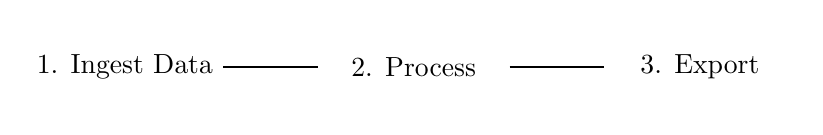
\begin{tikzpicture}[
    node distance=1.2cm,
    base/.style={
        rectangle, rounded corners, 
        minimum width=2.4cm, minimum height=1cm, 
        line width=1pt
    },
    % Define active and inactive styles separately
    node active/.style={draw=blue!80!black, fill=blue!10, text=blue!90!black},
    node inactive/.style={draw=gray!30, fill=gray!5, text=gray!35},
    arrow active/.style={-Latex, line width=1.2pt, draw=blue!80!black},
    arrow inactive/.style={-Latex, line width=1.2pt, draw=gray!25}
]
    % Apply the 'alt' key directly to nodes
    \node[base, alt=<1>{node active}{node inactive}] (n1) {1. Ingest Data};
    \node[base, alt=<2>{node active}{node inactive}, right=of n1] (n2) {2. Process};
    \node[base, alt=<3>{node active}{node inactive}, right=of n2] (n3) {3. Export};

    % Apply the 'alt' key directly to paths
    \draw[alt=<1-2>{arrow active}{arrow inactive}] (n1) -- (n2);
    \draw[alt=<2-3>{arrow active}{arrow inactive}] (n2) -- (n3);
\end{tikzpicture}
\end{frame}

\begin{frame}{Progressive Image Annotation}
\centering
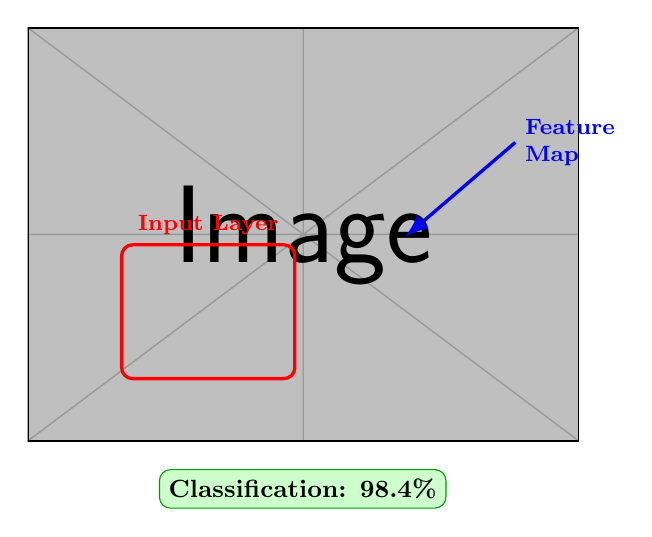
\begin{tikzpicture}
    % Base image: visible on all overlays (1+)
    \node[anchor=south west, inner sep=0pt] (img) at (0,0) {
        \includegraphics[width=7cm]{example-image}
    };

    % Overlay 2: Add a bounding box around a region
    \draw<2->[red, very thick, rounded corners] (1.2, 0.8) rectangle (3.4, 2.5);
    \node<2->[red, font=\footnotesize\bfseries, above] at (2.3, 2.5) {Input Layer};

    % Overlay 3: Add an arrow and label pointing to another part
    \draw<3->[-Latex, blue, very thick] (6.2, 3.8) -- (4.8, 2.6);
    \node<3->[blue, font=\footnotesize\bfseries, right, align=left] at (6.2, 3.8) {Feature\\Map};

    % Overlay 4: Add a final summary tag at the bottom
    \node<4->[fill=green!20, draw=green!60!black, rounded corners, font=\small\bfseries] 
        at (3.5, -0.6) {Classification: 98.4\%};
\end{tikzpicture}
\end{frame}

\begin{frame}{Cumulative Architecture Buildup}
\centering
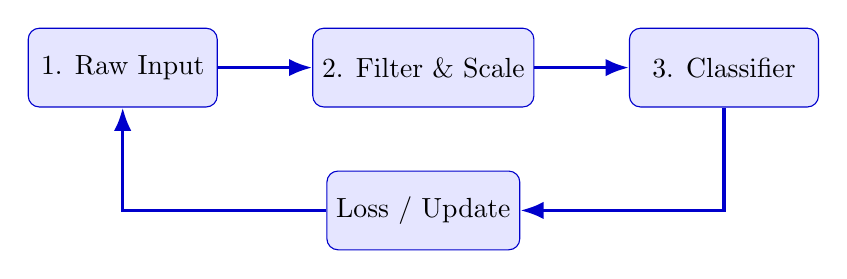
\begin{tikzpicture}[
    node distance=1.2cm,
    block/.style={
        rectangle, draw=blue!80!black, fill=blue!10, 
        rounded corners, minimum width=2.4cm, minimum height=1cm
    },
    conn/.style={-Latex, line width=1.2pt, draw=blue!80!black}
]
    % Step 1: Base node
    \node[block] (input) {1. Raw Input};

    % Step 2: Add processing stage and incoming connection
    \node[block, visible on=<2->, right=of input] (proc) {2. Filter \& Scale};
    \draw[conn, visible on=<2->] (input) -- (proc);

    % Step 3: Add classification stage and incoming connection
    \node[block, visible on=<3->, right=of proc] (out) {3. Classifier};
    \draw[conn, visible on=<3->] (proc) -- (out);

    % Step 4: Add feedback loop below the main flow
    \node[block, visible on=<4->, below=0.8cm of proc] (fb) {Loss / Update};
    \draw[conn, visible on=<4->] (out.south) |- (fb.east);
    \draw[conn, visible on=<4->] (fb.west) -| (input.south);
\end{tikzpicture}
\end{frame}

\begin{frame}{Progressive Buildup + Full Final Overview}
\centering
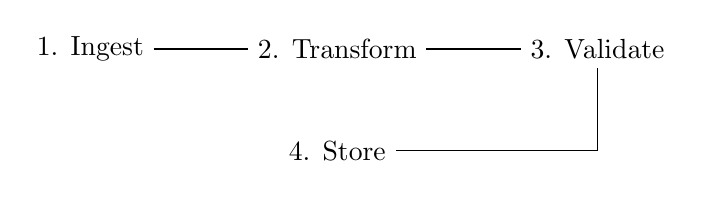
\begin{tikzpicture}[node distance=1.2cm]

    % Step 1: Active on 1 & 5 | Dimmed on 2, 3, 4
    \node[step node=1] (n1) {1. Ingest};

    % Step 2: Hidden on 1 | Active on 2 & 5 | Dimmed on 3, 4
    \node[step node=2, right=of n1] (n2) {2. Transform};
    \draw[step arrow=2] (n1) -- (n2);

    % Step 3: Hidden on 1-2 | Active on 3 & 5 | Dimmed on 4
    \node[step node=3, right=of n2] (n3) {3. Validate};
    \draw[step arrow=3] (n2) -- (n3);

    % Step 4: Hidden on 1-3 | Active on 4 & 5
    \node[step node=4, below=0.8cm of n2] (n4) {4. Store};
    \draw[step arrow=4] (n3.south) |- (n4.east);

\end{tikzpicture}
\end{frame}

\begin{frame}{Step-by-Step Image Annotations}
\centering
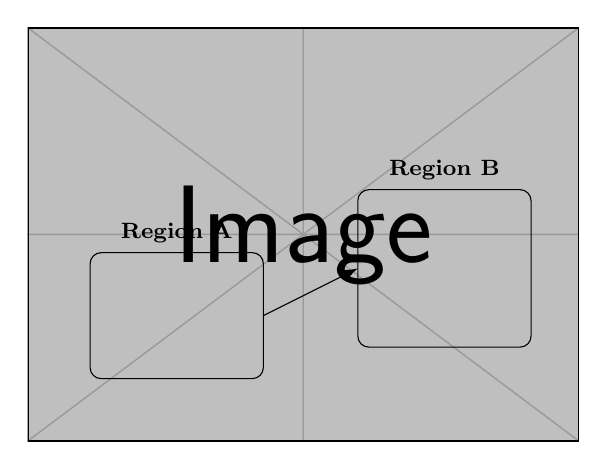
\begin{tikzpicture}
    % Static base image
    \node[anchor=south west, inner sep=0pt] at (0,0) {
        \includegraphics[width=7cm]{example-image}
    };

    % Annotation 1: Highlighted on Slide 1, dimmed on Slide 2+
    \draw[box focus=1, rounded corners] (0.8, 0.8) rectangle (3.0, 2.4);
    \node[box focus=1, above, font=\footnotesize\bfseries] at (1.9, 2.4) {Region A};

    % Annotation 2: Appears active on Slide 2, dimmed on Slide 3+
    \draw[box focus=2, rounded corners] (4.2, 1.2) rectangle (6.4, 3.2);
    \node[box focus=2, above, font=\footnotesize\bfseries] at (5.3, 3.2) {Region B};

    % Annotation 3: Appears active on Slide 3
    \draw[box focus=3, -Latex] (3.0, 1.6) -- (4.2, 2.2);
\end{tikzpicture}
\end{frame}


\appendix

\section{Appendix}

\begin{frame}{Appendix}
    This is an appendix.
    \begin{itemize}
        \item Page numbers start from the beginning.
    \end{itemize}
\end{frame}

\end{document}
